\documentclass{article} 

% importar paket, kommandon och annat från "preamble.sty" där allt är samlat
\usepackage{init}
\usepackage{amsmath}
\usepackage[⟨options⟩]{fancyhdr}
\usepackage[colorlinks=true, urlcolor=blue, linkcolor=black]{hyperref}
\begin{document}
    \selectlanguage{swedish}
    \pagestyle{fancy}
%... then configure it.
\fancyhead{ESSF20- Komponentfysik/ Physics of Devices} % clear all header fields
\fancyhead[RO,L]{{}}

% skapar titelsidan, ligger i ett .tex dokument i mappen "titlepage". Finns flera versioner att använda sig av genom att kommentera ut/in 
    % @Depricated - bilden är inte genomskinlig
% logo i mitten ovanför titeln med "lunds tekniska högskola" under
% 
\includegraphics[scale=0.3]{tp/lth_transparent_tekniska.png}
% \vspace*{1cm}

% logo i mitten ovanför titeln
% \begin{tikzpicture}[remember picture,overlay]
%     \node[anchor=north,inner sep=0pt] (logo) at (current page.north) {
\includegraphics[scale=0.4]{tp/lth_transparent_notext.png}}; 
%     % \node [below=-25pt of logo] {\textbf{text}};
% \end{tikzpicture}
% \vspace*{5cm}

% logo i mitten ovanför titeln med "lunds universitet" under
% \begin{tikzpicture}[remember picture,overlay]
%     \node[anchor=north,inner sep=0pt] (logo) at (current page.north) {
\includegraphics[scale=0.3]{tp/lth_transparent.png}}; 
%     % \node [below=-25pt of logo] {\textbf{text}};
% \end{tikzpicture}
% \vspace*{6cm}

%lth-logo i övre högra hörnet, med text under
% \begin{tikzpicture}[remember picture,overlay]
%     \node[anchor=north west,inner sep=0pt] (logo) at (current page.north west) {
\includegraphics[scale=0.4]{tp/lth_transparent_notext.png}}; 
%     % \node [below=-25pt of logo] {\textbf{text}};
% \end{tikzpicture}
% \vspace{3cm}

% % lth-logo i nedre högra hörnet
\begin{tikzpicture}[remember picture,overlay]
    \node[anchor=south east,inner sep=0pt] (logo) at (current page.south east) {
\includegraphics[scale=0.55]{tp/lth_transparent_corner.png}}; 
    % \node [below=-25pt of logo] {\textbf{text}};
\end{tikzpicture}

% % stil 1 av texten
\begin{center}
    \textbf{\huge Komponentfysik - ESSF20}
    
    \vspace{0.8cm}
        
    \vspace{0.8cm}

    \vspace{0.3cm}
    \textbf{Walter Mundt-Petersen}    \\
    Shoutout till Rydbergssalen, mobilspel, och Khan Academy.
    \vfill
        
    \vspace{0.8cm}
    
    
    LTH\\
    Lunds Universitet\\
    Sverige\\
    \today % skriver in dagens datum
\end{center}


% stil 2 av texten
% \begin{center}
%     \parbox{5cm}{
%         \begin{flushleft}
%             \huge 
%             Labbrapport \\
%             \vspace{0.25cm}
%             \large 
%             Version nr: 3 \\
%             \vspace{0.7cm}
%             Lab: Impedans
%         \end{flushleft}
%         }
% \end{center}

% \vfill
% \begin{flushleft}
%     \large
%     Handledare: Elin Dahlgren \\
%     \vspace{0.65cm}
%     Laboration utförd datum: \today\\
%     \vspace{0.65cm}
%     Utförd av: Marcel Martens \& Jonathan Carlsson \\
%     Grupp nr: 24\\
%     \vspace{0.65cm}
%     Granskad av: Mattias Lindskoug \& Vincent Olson \\
%     Grupp nr: 21\\
% \end{flushleft}

% % Lägger till table of contents och rensar resten av sidan
\break
\clearpage
\section{Atomfysik} 



\footnote{Videor relevanta till kapitel \ref{sec:atomfysik}: \href{https://www.youtube.com/playlist?list=PL2ub1_oKCn7ogaMtdB2RumlIYqNeXf_oX}{Khan Academy, Semiconductors, videor 1-4.}}
\label{sec:atomfysik}
Pauli's Exclusion Principle states that no two electrons in the same atom can have identical values for all four of their quantum numbers. In other words, (1) no more than two electrons can occupy the same orbital and (2) two electrons in the same orbital must have opposite spins

\begin{figure}[ht]
    \centering
    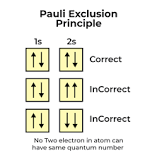
\includegraphics{bilder/fig:pauli.png}
    \caption{Pauli's exclusion principle}
    \label{fig:paulis}
\end{figure}

\begin{itemize}
    \item Bra ledare $\implies$ Många fria elektroner.
    \item Halvledare $\implies$ Väldigt få fria elektroner.
    \item Isolatorer $\implies$ I princip 0 fria elektroner.
\end{itemize} 

\subsection{Energinivåer}
Enligt Pauli kan inga två atomer ha samma energinivå. Dock kan en atom ha positiv eller negativ 'spinn' och då kan 2 elektroner få plats på samma energinivå, visat nedan i figur \ref{fig:Energinivåer}.

\begin{figure}[ht]
    \centering
    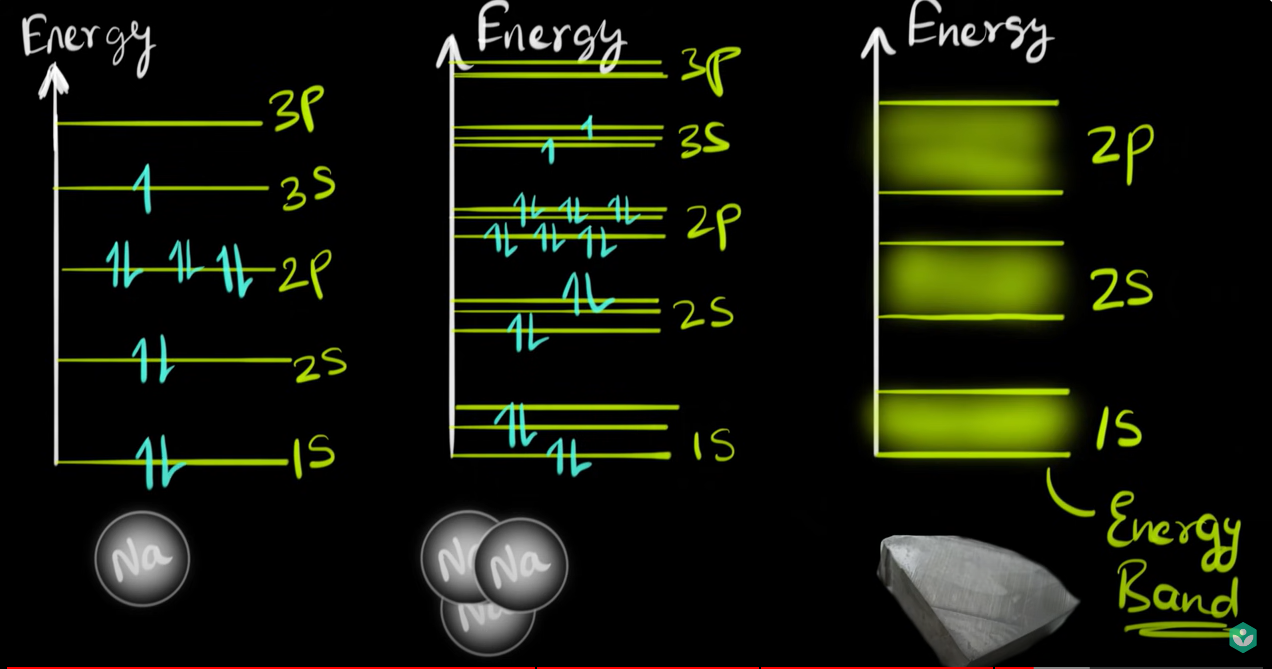
\includegraphics[scale = 0.3]{bilder/fig:energi.png}
    \caption{Energinivåer}
    \label{fig:Energinivåer}
\end{figure}

Ovan ser man visuellt hur en Natriumatoms energikonfiguration ser ut. De blåa pilarna är en atom vardera, med spinn åt olika håll. Olika nivåer (1S, 2S, 2P...) får plats med olika många atomer. Andra grafen visar hur en natriummolekyls elektronkonfiguration ser ut. Som man ser i andra grafen skapas flera orbitalnivåer på varje steg (1S, 2S, 2P...). Dessa brukar kallas 1S*, 2S* osv. Kombinationen av streck på varje orbitalnivå i andra grafen föreställer de nyskapade orbitalnivåerna för en molekyl. I fasta material har vi en enormt hög koncentration av atomer, vilket således leder till enormt många orbitalnivåer på varje steg 1S, 2S... Detta illustreras i grafen till höger. Vad som i den grafen är ritat som ett 'moln' är egentligen enormt många individuella orbitalnivåer, allt enligt Paulis princip (\ref{sec: pauli}). Detta 'moln' kallas för 'energiband'. Eftersom att varje energinivå kan hålla 2 elektroner (positiv och negativ spinn), kan varje energiband med \textit{N} antal energinivåer bära \textit{2N} antal elektroner.

Varje orbital 1S, 2S... kan hålla olika antal elektroner. 
\begin{itemize}
    \item s-orbital: Varje s-orbital kan hålla upp till 2 elektroner.
    \item p-orbital: Varje p-undernivå kan hålla upp till 6 elektroner (3 olika orbitaler, var och en med plats för 2 elektroner).
    \item d-orbital: Varje d-undernivå kan hålla upp till 10 elektroner (5 olika orbitaler, var och en med plats för 2 elektroner).
    \item f-orbital: Varje f-undernivå kan hålla upp till 14 elektroner (7 olika orbitaler, var och en med plats för 2 elektroner).
\end{itemize}

\begin{figure}[ht]
    \centering
    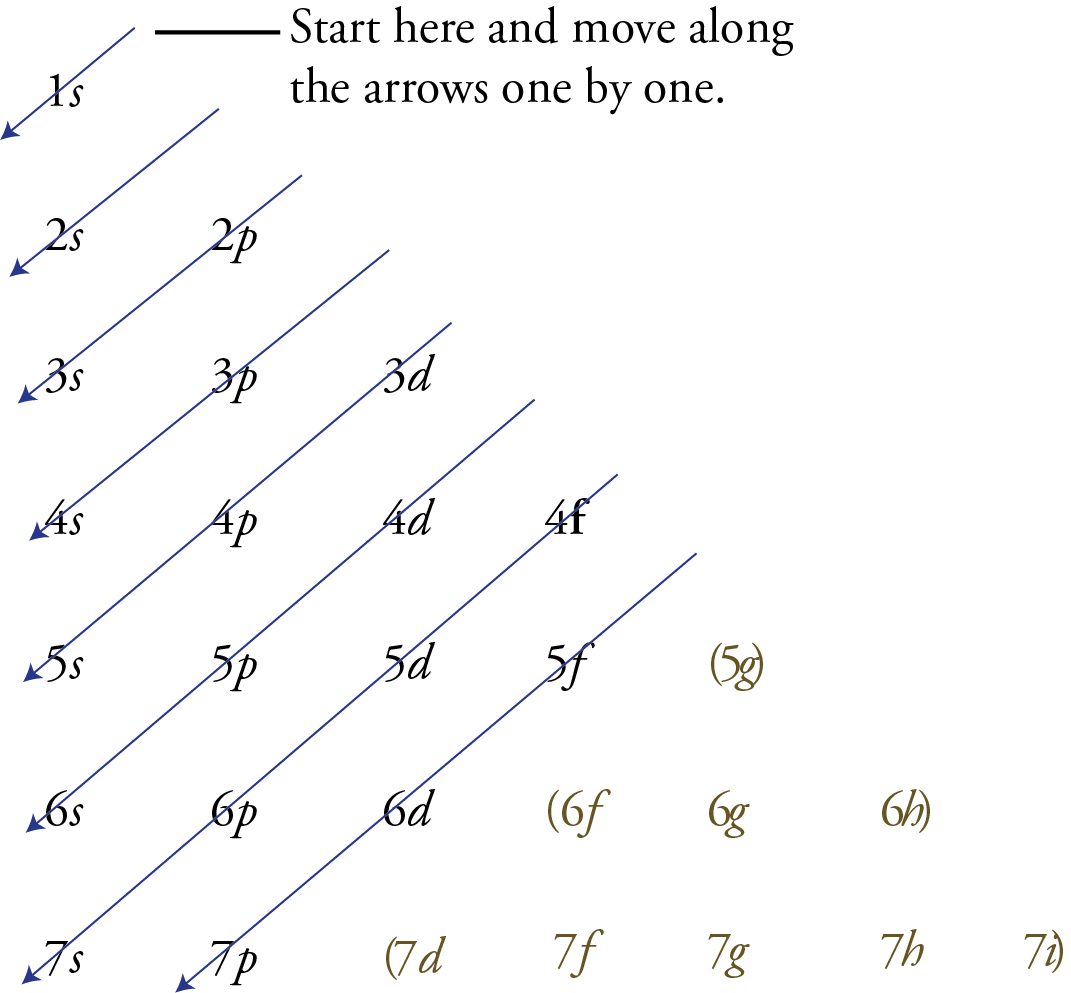
\includegraphics{bilder/fig:elektronkonfig.png}
    \caption{Orbitalnivåer och dess förmåga att hålla elektroner.}
    \label{fig:orbitalnivåer}
\end{figure}

Varje streck i figur \ref{fig:Energinivåer} visar ett atomskal i ordning K,L,M,N där om man summerar antalet elektroner varje orbitalnivå kan hålla kommer fram till att de respektive skalen kan hålla 2, 8, 18, 32 elektroner. Exempelvis kan alltså 'strecket' som går över 3d, 4p, 5s bära $10 + 6 + 2 = 18$ elektroner. Det strecket representerar således ett M-skal.



Det krävs energi för en elektron att kunna röra sig mellan orbitalnivåer. En temperaturökning kan vara någonting som tillför denna energin. I material som vi kallar för ledare, överlappar orbitalnivåerna varandra, och gapet, $E_g$, försvinner. Istället får vi ett enda stort band där elektroner kan röra sig fritt, vilket illustreras i den vänstra grafen i figur \ref{fig: valens_ledningsband}. För isolatorer är detta bandgap väldigt stort villket försvårar elektronrörelse, och för halvledare är det lite mittemellansvårt. Ledare, isolatorer, och halvledare definieras utifrån storleken på detta gap enligt följande:

\begin{equation}
    \begin{cases}
       & {Ledare: E_g < 0 eV} \\
       & {Halvledare: 0 eV < E_g < 2 eV} \\
       & {Isolatorer: E_g > 4 eV}
    \end{cases}       
\end{equation}

Dessa definitionerna lämnar lite utrymme vad gäller energinivåer som krävs för elektronövergång men jag gissar att man inte vill använda de materialen bara för att de är både kassa halvledare \textit{och} kassa isolatorer.

Valensband är definierat som det högsta fyllda bandet vid 0 K (måste inte vara helt fyllt). Det näst högsta bandet heter ledningsbandet. För en ledare har man bara ett stort band, därför kallar man det oftast inte för något av valens/ledningsband. 

\begin{figure}[ht]
    \centering
    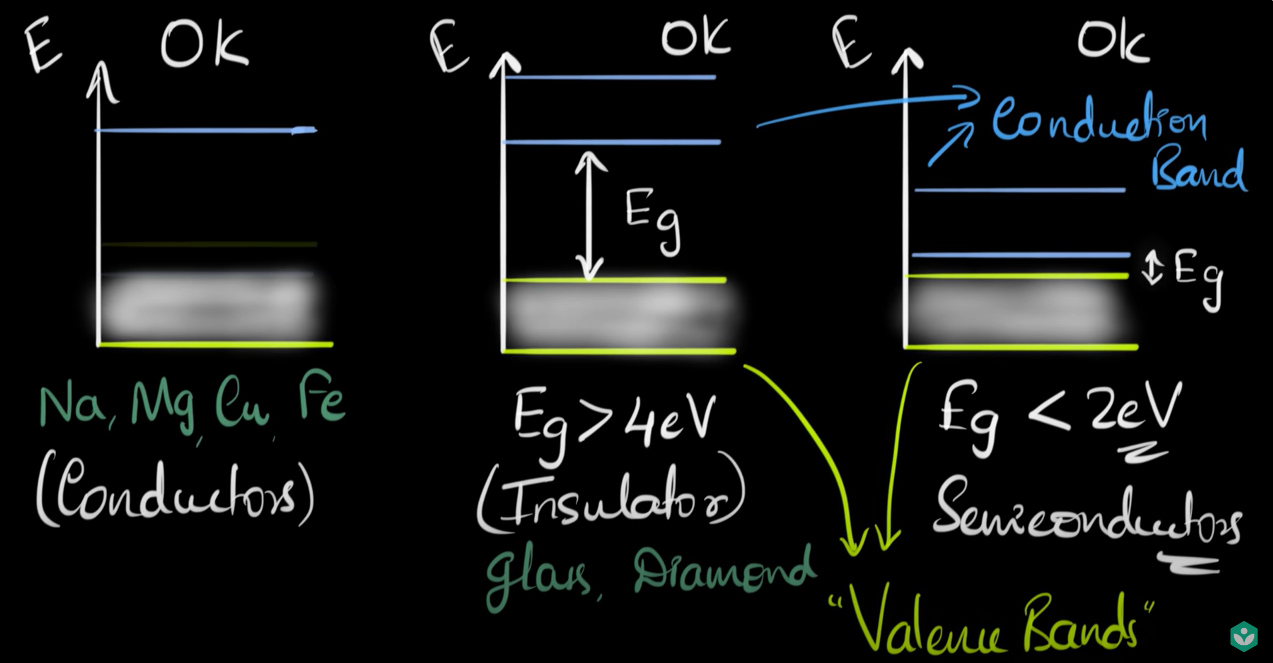
\includegraphics[scale = 0.3]{bilder/gap_iso_halvledare_ledare.PNG}
    \caption{Valensband och ledningsband för ledare, isolatorer, och halvledare.}
    \label{fig: valens_ledningsband}
\end{figure}


\section{Halvledare} 

\footnote{Videor relevanta till kapitel \ref{sec:halvledare}: \href{https://www.youtube.com/playlist?list=PL2ub1_oKCn7ogaMtdB2RumlIYqNeXf_oX}{Khan Academy, Semiconductors, videor 5-9.}}
\label{sec:halvledare}
Halvledare kallas det för att de kan både leda, och isolera\footnote{Fräckt!}. Vid låg temperatur kommer halvledaren att isolera och vid hög temperatur kommer den att leda bättre. Vad som är hög och låg temperatur är unikt för varje enskilt ämne. När man ökar temperaturen kring en halvledare och dess ledningsförmåga ökar, kommer elektronerna i ämnet att börja hoppa från det helt fyllda valensbandet över till ledningsbandet. En elektron som hoppar till ledningsbandet (eller tvärtom) lämnar ett hål bakom sig på platsen den lämnade. Dessa hål är inte partiklar men det är intuitivt att se dem som partiklar som rör sig i motsatt riktning från elektronernas rörelse. Föreställ dig en nästan fylld vattenflaska med en luftbubbla i sig. Håller du flaskan upprätt kommer allt vatten sjunka till botten (och luftbubblan lägger sig överst i flaskan). Vänder du flaskan upp och ner kommer allt vatten att lägga sig vid flaskans lock, och luftbubblan lägga sig vid flaskans botten (numera ovansidan). Luftbubblans rörelse provoceras som en följd av vattnets rörelse. 
\begin{figure}[ht]
    \centering
    
\includegraphics[scale = 0.3]{bilder/vatten.png}
    \caption{Flaska, möjligtvis av glas, fylld med genomskinlig vätska.}
    \label{fig:vatten}
\end{figure}

\subsection{Extrinsiska halvledare, doping}

\textbf{Definition:} En halvledare kallas 'intrinsisk' om alla atomer är av samma ämne \footnote{Intrinsiska halvledare kallas ibland 'pura' halvledare.}. Motsatsen gäller även, alltså; en halvledare bestående av mer än ett ämne kallas 'extrinsiska'.

Då du kombinerar två ämnen kommer det att påverka dess elektronstruktur. Mellan den intrinsiska halvledarens valensband och ledningsband kommer en ny möjlig energinivå att dyka upp. Elektroner kan hoppa till denna nya energinivå. Är den nya nivån nära valensbandet kommer den att uppmuntra elektronerna i valensbandet att hoppa dit, och således lämna hål efter sig i valensbandet. Vice versa gäller för om den nya energinivån ligger nära ledningsbandet.

För en p-typ halvledare kallas den nyuppståndna energinivån acceptornivå. Om du dopar din halvledare med ett ämne som ligger i atomgruppen nedanför kommer acceptornivån ligga precis ovanför valensbandet, vilket gör det sannolikt för elektroner att hoppa dit. Ju längre ner i atomgrupperna du går, desto längre bort från valensbandet hamnar denna acceptornivå, och minskar alltså den önskade effekten av att skapa hål i valensbandet.

Motsvarande gäller även för n-typ halvledare, fast ju längre uppåt i atomgrupperna du vandrar, desto närmare valensbandet kommer du med acceptornivån, vilket minskar valensbandets elektronkoncentration, alltså motsatt från önskad effekt.

T.ex kisel tillhör atomgrupp 14. Kombinerar du kisel med ett ämne från atomgrupp 15, alltså med en elektron mer än kisel, kommer den atomen, efter sina kovalenta bindningar, ha en elektron över som inte är bunden. Den elektronen är fri. Detta kommer leda till ett 'överflöd' av elektroner i valensbandet, och ämnets ledningsförmåga ökar avsevärt. Ämnet med många elektroner kallas för en 'n-typ halvledare'.

Omvänt gäller; om du dopar ett ämne (gör ämnet extrinsiskt) med ett ämne från atomgruppen under, så kommer det att skapas en stor mängd hål i valensbandet, vilket 

\subsection{PN-övergång}

Då två p-dopade resp. n-dopade halvledare sätts ihop bildas en PN-övergång. Området i mitten av de två halvledarna kallas för spärrskikt, där de respektive majoritetsladdningsbärarna tar ut varandra i vad som kallas rekombination. Med hjälp av en PN-övergång och manipulation av dess spärrskikt kan man få PN-övergången att fungera som en diod.

\subsection{Dioder}
Denna ovannämnda manipulation består av att 'framspänna' PN-övergången. Detta innebär att man tillför en spänningskälla, en förspänning, vars positiva sida är kopplad till PN-föreningens (diodens) positiva sida, och motsvarande för de negativa sidorna. Då källans spänning ökar kommer spärrskiktet kontinuerligt att minska tills det inte finns längre, och dioden fungerar då som en väldigt bra ledare. Spänningen då spärrskiktet är minskat till noll kallas för diodens tröskelspänning. Man kan även invertera källans poler och då 'backspänna' dioden. Man kan även säga att man 'biaserar' dioden (positivt eller negativt).

Om du byter backspänner dioden kommer du uppnå motsatt effekt, alltså att spärrskiktet bara ökar i storlek. Slutsatsen blir att dioden bara släpper igenom ström då spänningen har 'rätt' polaritet, vilket ger oss en mycket användbar komponent i kretsdesign, till exempel vid implementering av \href{https://sv.wikipedia.org/wiki/Likriktning}{likriktare}.

\begin{figure}[ht]
    \centering
    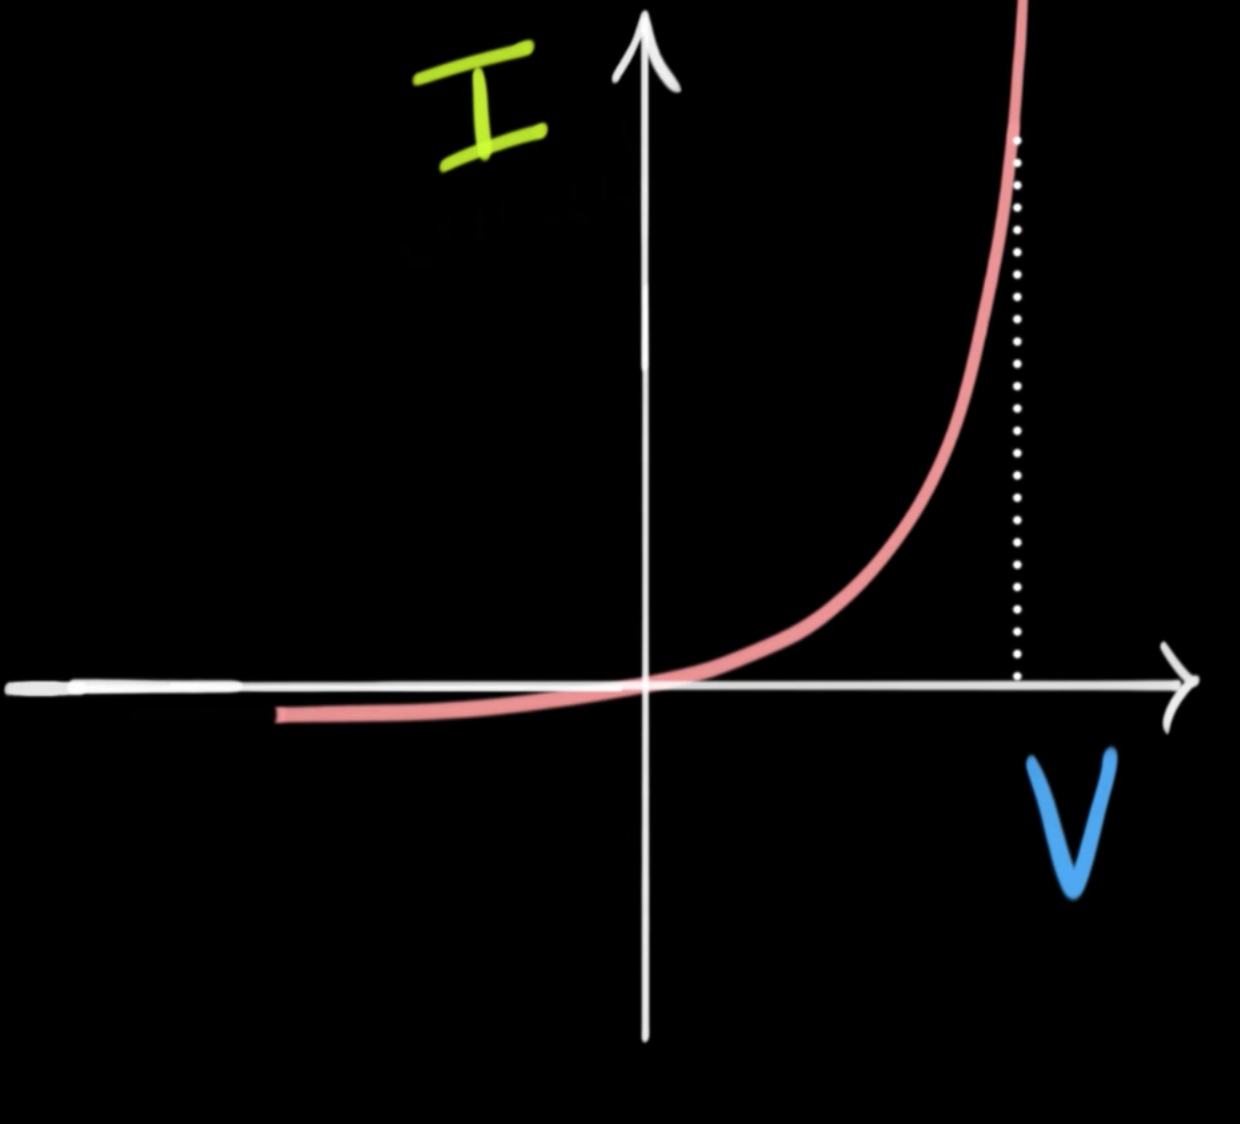
\includegraphics[scale = 0.3]{bilder/fig: arbetspunkt.png}
    \caption{Ström som flödar genom en diod plottat mot dess förspänning. Vita punkterna visar diodens arbetspunkt, dess tröskelspänning.}
    \label{fig:arbetspunkt}
\end{figure}

\newpage

Resten av kursen består av elektronik kopplat till transistorer. Jag har inte mer tid och förhoppningsvis har du lärt dig hur en transistor fungerar någorlunda i tidigare elektronikkurser, därför kommer jag för denna gång att avsluta sammanfattningen av denna fina kurs här! 


    

\end{document}
